% =====================================================================
%  ISE XAI Group 10 — Short paper (IEEE two-column conference format)
%  Plan: plans/2026-10-18-paper-plan.md
%  Each section lives in its own file in sections/. 
% =====================================================================
\documentclass[conference]{IEEEtran}
\IEEEoverridecommandlockouts
\usepackage{cite}
\usepackage{amsmath,amssymb,amsfonts}
\usepackage{graphicx}
\usepackage{booktabs}
\usepackage{xcolor}
\usepackage{url}
\usepackage{flafter}   % a figure/table never appears before its place in the text (stops Results floats landing above Sec. IV)
\graphicspath{{figures/}}

\DeclareRobustCommand{\todo}[1]{\textcolor{magenta}{[TODO: #1]}}   % robust so it also works inside captions

\begin{document}

\title{Do Attributions Tell the Truth About Data Filters?\\[0.2em]
{\Large Measuring the Faithfulness of SHAP and LIME in Identity-Term Bias Audits}}

\author{
\IEEEauthorblockN{Julia Hooper, Bl\'aith\'in Kavanagh, Rory Linnane and April Gilhool}
\IEEEauthorblockA{\textit{University of Limerick}}
}

\maketitle

\begin{abstract}
% ---------------------------------------------------------------------
% ABSTRACT (about 150 words)
% main.tex already wraps this file in \begin{abstract}...\end{abstract},
% so this file holds plain text only. No citations (IEEE style).
% Every number is from Results (Sec. IV) / Table I.
% Owner April Gilhool
% ---------------------------------------------------------------------
Pretraining data filters silently decide whose language large language models learn from, and have been shown to remove text from specific groups. They are audited only in aggregate, and nobody has checked whether the feature-attribution explanations an auditor would use to explain individual removals are faithful. We test SHAP and LIME on the Detoxify toxicity filter against two references whose answers can be computed independently, counterfactual identity-word swaps and exact Shapley values on a transparent filter, plus a deletion test and a stability test. Both explainers rank identity-word effects almost as the counterfactual does (Spearman $\rho = 0.96$ for SHAP, 0.97 for LIME) and recover exact Shapley values ($\rho \geq 0.98$), but SHAP overstates the size of the effect, and its error depends on how removed words are replaced. On weak signals LIME's surrogate fit falls ($R^2$ 0.77 to 0.41), and SHAP--LIME disagreement is no better than chance (AUC 0.46) at flagging wrong explanations. Attribution can therefore triage a filter for identity-term bias, but cannot certify it as fair.

\end{abstract}

\begin{IEEEkeywords}
explainable AI, feature attribution, SHAP, LIME, faithfulness, pretraining data filters, social bias
\end{IEEEkeywords}

% ---------------------------------------------------------------------
% I. INTRODUCTION (about 0.4 page)
% Owner: ___
%
% ---------------------------------------------------------------------
\section{Introduction}\label{sec:intro}

\todo{Introduction, about 0.4 page. }

% ---------------------------------------------------------------------
% II. BACKGROUND AND RELATED WORK (about 0.5 page)
% Owner: Rory Linnane
%
% ---------------------------------------------------------------------
\section{Background and Related Work}\label{sec:background}

\subsection{Bias in Pretraining Data Filters}
Large language models are trained on web-scale corpora filtered through pipelines that silently encode value judgements.
Dodge et al.\ showed that C4's word blocklist disproportionately removes text by and about LGBTQ+ people and in African American English (AAE)~\cite{dodge2021documenting}.
Quality filters compound this: Gururangan et al.\ found that a replica of GPT-3's quality filter assigns higher scores to text from wealthier, urban and more educated sources~\cite{gururangan2022whose}.
Toxicity classifiers exhibit the same pattern: Sap et al.\ showed hate-speech detectors flag AAE at significantly higher rates than equivalent white-aligned English~\cite{sap2019risk}, and Mendu et al.\ found that a transformer-based filter misclassifies news articles that \emph{report} on harmful content as harmful themselves~\cite{mendu2025safer}.
Fairness-oriented filters are not immune: Udagawa et al.\ found a regard classifier removes sentences that report real-world events involving marginalised groups~\cite{udagawa2025bias}.
Identity-term templates offer a controlled way to probe these failures.
Dixon et al.\ introduced the minimal-pair method, which substitutes one identity word for a neutral control (e.g.\ ``my neighbour is \emph{gay}'' vs.\ ``my neighbour is \emph{tall}'') to isolate unintended classifier bias~\cite{dixon2018measuring}.
Borkan et al.\ extended this work to real comments, releasing the identity-labelled Civil Comments data on which Detoxify \texttt{unbiased} was later trained~\cite{borkan2019nuanced}.
However, across all filter types, these audits measure only aggregate removal rates by group, and none explains why an individual sentence was removed.

\subsection{Feature Attribution for Text}
Post-hoc feature attribution assigns each input token a score reflecting its contribution to the model's prediction, without modifying the model itself.
SHAP grounds attribution in cooperative game theory: Lundberg and Lee showed that the Shapley value, the unique attribution satisfying efficiency, symmetry and the null-player axiom, can be computed for any model via a unified additive framework~\cite{lundberg2017unified}.
For text, the SHAP library uses a partition approximation; exact Shapley enumeration is feasible only for short sequences, which allows it to serve as a reference (Sec.~\ref{sec:method}).
LIME takes a complementary approach: Ribeiro et al.\ fit a locally weighted sparse linear surrogate to random perturbations of the input, measuring local fidelity through the surrogate's $R^2$~\cite{ribeiro2016why}.
Both methods are post-hoc, local (one prediction at a time) and model-agnostic: they treat the classifier as a black box and require only query access~\cite{munn2022xai}.

\subsection{Evaluating Explanations: Faithfulness vs.\ Agreement}
Jacovi and Goldberg define an explanation as \emph{faithful} if it correctly describes the model's actual reasoning process, and distinguish this from whether it looks plausible to a human~\cite{jacovi2020faithfully}.
Deletion-based metrics operationalise faithfulness: DeYoung et al.'s ERASER benchmark defines \emph{comprehensiveness} (the score drops when the top-$k$ attributed tokens are deleted) and \emph{sufficiency} (the score is preserved when only those tokens are kept)~\cite{deyoung2020eraser}.
These metrics have a known limitation: deleting words produces inputs outside the model's training distribution, so score changes may partly reflect distributional shift rather than token importance~\cite{hase2021ood}.
More broadly, post-hoc explainers are imperfect.
Krishna et al.\ showed that SHAP and LIME frequently disagree on feature rankings for the same input, so agreement between them does not imply either is correct~\cite{krishna2022disagreement}.
Slack et al.\ demonstrated that explanations can be adversarially manipulated to conceal discriminatory model behaviour~\cite{slack2020fooling}.
Ngueajio et al.\ found that the highest-accuracy classifier is not necessarily the one whose explanations are most faithful~\cite{ngueajio2025decoding}.
These evaluations were conducted on general classification tasks; to our knowledge, no prior work has evaluated attribution faithfulness in pretraining filter audits against references whose correct answers are known independently.

% ---------------------------------------------------------------------
% III. METHOD (about 0.6 page)
% Owners: one paragraph per experiment owner: ___
%
% FACTS lists below were checked against the notebooks (*.ipynb), the
% results CSVs and the journal. Source in [brackets] after each fact.
% "nb" = notebook. Where a fact could NOT be confirmed it says CHECK.
% ---------------------------------------------------------------------
\section{Method}\label{sec:method}

\subsection{Filters}
% PLAN: which filters did we test?
% - Detoxify "original" and Detoxify "unbiased".
% - Note: they are different model types (BERT vs RoBERTa), not just
%   debiased vs not debiased.
% - Our own simple, transparent filter built for Exp 4 (a logistic
%   regression on words and word pairs), and how accurate it is compared
%   with Detoxify (numbers in Exp 4's exp4_auc.csv).
%
% FACTS:
% - Detoxify models: "original" and "unbiased" [all nbs, Cell 1]
% - Output used: the "toxicity" score, P(toxic) [all nbs, proba()]
% - Converted to log-odds for SHAP: log(p / (1 - p)), p clipped to
%   1e-6 .. 1 - 1e-6 [all nbs, logit()]
% - Mask tokens: "[MASK]" for original, "<mask>" for unbiased
%   [Exp 3 nb, Cell 9] -> fits BERT vs RoBERTa
% - BERT vs RoBERTa: [journal, Dixon 2018 note] -- CHECK against the
%   Detoxify README (cite key: detoxify); not stated in the notebooks
% - "unbiased" was trained for the Jigsaw Unintended Bias competition,
%   i.e. on Civil Comments [Exp 4 nb, Cell 4 caveat; journal, Borkan 2019
%   note] -> cite borkan2019nuanced
% - Transparent filter [Exp 4 nb, Cells 2-3]:
%   - dataset: Civil Comments (google/civil_comments, Hugging Face)
%   - toxic = toxicity >= 0.5
%   - training: 100,000 comments sampled from the train split (seed 42)
%   - features: binary word counts, words that appear in >= 5 comments
%   - main filter: words + word pairs (unigrams + bigrams)
%   - sanity-check filter: single words only
%   - model: logistic regression (C = 1.0)
% - Accuracy, AUC on 5,000 test comments (seed 42) [exp4_auc.csv]:
%   - transparent, words + pairs: 0.892
%   - transparent, words only: 0.897
%   - Detoxify original: 0.928
%   - Detoxify unbiased: 0.971 (favoured: trained on this dataset)

\todo{Detoxify original and unbiased, plus the transparent filter (Exp 4).}

\subsection{Sentence Sets}
% PLAN: what sentences did we feed the filters?
% - Exp 1: 48 sentences that use the same insult in three ways
%   (promoting, reporting, arguing against).
% - Exp 2: 190 harmless sentences where only one word changes
%   (an identity word like "gay", or a neutral word like "tall").
%   Based on Dixon 2018.
% - Exp 4 also uses 200 real comments from Civil Comments.
% - The other experiments reuse these same sentences.
%
% FACTS:
% - Exp 1 set: 48 sentences = 16 topics x 3 versions [Exp 1 nb, Cell 2;
%   exp1_results.csv has 48 rows]
%   - promote / report / counter, same insult words in all 3
%   - example (topic 1): "Those fans are disgusting idiots and should be
%     banned." / "The club condemned a post calling its fans disgusting
%     idiots who should be banned." / "Calling the fans disgusting idiots
%     is unfair and wrong."
%   - report sentences are longer than the others [Exp 1 nb, Cell 2
%     comment] -> limitation
% - Exp 2 set: 190 sentences = 10 harmless templates x 19 words
%   [Exp 2 nb, Cell 2; exp2_results.csv has 190 rows]
%   - 15 identity words: gay, lesbian, transgender, black, white, asian,
%     muslim, jewish, christian, immigrant, deaf, blind, disabled, poor,
%     rural
%   - 4 control words: tall, young, local, quiet
%   - 150 identity sentences + 40 control sentences
%   - example template: "My best friend is {}."
%   - design follows Dixon 2018 [journal, Dixon 2018 note] -> cite
%     dixon2018measuring
% - Exp 4 set: 438 sentences [exp4_sentences.csv]
%   - the 48 Exp 1 + 190 Exp 2 sentences
%   - plus 200 real comments: 100 toxic, 100 non-toxic, 5-14 words,
%     from the full Civil Comments test split (seed 42) [Exp 4 nb, Cell 6]
%   - cap of 16 tokens; all 438 were under it, none removed
% - Which experiment uses which set [nbs, Cell 2 of each]:
%   - Exp 3: the 190 Exp 2 sentences
%   - Exp 5 and Exp 6: all 238 Exp 1 + Exp 2 sentences

\todo{Exp 1, Exp 2, and the Exp 4 real comments.}

\subsection{Explainers}
% PLAN: how did we set up SHAP and LIME?
% - SHAP: which version we used and its main setting.
% - LIME: how many samples and that we fixed the random seed.
% - Both explain each word's effect on the "toxic" score.
% - When an explainer "removes" a word, something has to replace it.
%   Say what we used, and that Exp 3 tests other options.
% - Careful: the settings are not the same in every experiment
%   (Exps 1-2 used fewer samples than Exps 3-6). Check the notebooks.
%
% FACTS:
% - All run on Google Colab, T4 GPU; libraries detoxify, shap, lime
%   [all nbs, Cell 0-1]; random seed 42 [all nbs]
% - Units: whole words, keeping attached punctuation, so SHAP and LIME
%   score the same words [Exps 1, 3-6 nbs, word_tokenizer()]
%   - Exp 2 split on spaces instead [Exp 2 nb, Cell 1]; Exp 3 re-ran
%     Exp 2's sentences with the word-level version [Exp 3 nb]
% - SHAP [all nbs]:
%   - shap.Explainer with a text masker -> Partition explainer (Exp 4
%     names "partition" explicitly)
%   - explains log-odds of toxic (so values add up)
%   - max_evals = 500 (Exp 2: 300)
%   - efficiency check after every Detoxify run: base value + sum of
%     SHAP values must equal the log-odds within 0.01, or the notebook
%     stops [all nbs, check_efficiency()]
%   - deterministic: Exp 2 compares two SHAP runs [Exp 2 nb, Cell 8]
%     -- CHECK: the printed result was not saved in the notebook
% - LIME [all nbs, lime_word_weights()]:
%   - LimeTextExplainer, labels = (1,) so weights are for "toxic"
%   - explains the probability, not log-odds -> only compared by rank
%     with SHAP
%   - one feature per distinct word, so no word is cut off
%   - samples and seeds per experiment:
%     - Exp 1: 2000 samples, seed 42
%     - Exp 2: 2000 samples, seed 42 (agreement on 40 sentences); 500
%       and 5000 samples x seeds 0-9 (stability tests)
%     - Exp 3, Exp 5: 5000 samples, seed 42
%     - Exp 4: 5000 samples, seeds 0-9
%     - Exp 6: 500 and 5000 samples, seeds 0-9
% - Removal baseline (what replaces a "removed" word):
%   - SHAP default: "..." [Exp 3 nb, Cell 9 note says "..." is shap's
%     default and what Exps 1-2 used] -- CHECK: the printed value was not
%     saved in the notebook
%   - Exp 3 also tests: deleting the word (a single space, because an
%     empty string crashes shap) and the model's mask token ("[MASK] " /
%     "<mask> ") [Exp 3 nb, Cell 9]
%   - Exp 4: deletion, for both SHAP and the exact values [Exp 4 nb]
%   - Exp 5's deletion test deletes words [Exp 5 nb, drop()]
% - Which model each experiment explains:
%   - both Detoxify models: Exps 1-3 SHAP, Exp 3 LIME, Exp 5
%   - original only: Exp 1-2 LIME, Exp 6
%   - transparent filter only: Exp 4

\todo{SHAP and LIME configuration, log-odds, removal baseline.}

\subsection{References}
% PLAN: what "right answers" did we compare the explainers against?
% - Counterfactual effect (Exp 3): swap the identity word for a neutral
%   word and see how much the score changes. Only one word differs, so
%   that change is the word's real effect.
% - Exact Shapley values (Exp 4): on our transparent filter we can work
%   out the exact correct answer, then see if SHAP and LIME match it.
% - Why we need these: two explainers agreeing doesn't prove they are
%   right (Krishna 2022).
%
% FACTS:
% - Counterfactual effect [Exp 3 nb, Cell 5]:
%   - for each of the 150 identity sentences
%   - = its log-odds minus the mean log-odds of the 4 control sentences
%     from the same template
%   - SHAP's estimate to compare = the identity word's SHAP value minus
%     the mean SHAP value of the control words in the same template
%   - "spill-over" = counterfactual effect minus SHAP's estimate (the
%     part SHAP put on other words)
%   - for LIME: the same, but in probability [Exp 3 nb, Cell 6]
%   - counterfactual swap method -> cite garg2019counterfactual
%     (in refs.bib; no journal review yet)
% - Exact Shapley values [Exp 4 nb, Cell 7]:
%   - on the transparent filter only
%   - players = the same word tokens SHAP uses
%   - value of a subset = the filter's log-odds with all other words
%     deleted
%   - every subset is tried (2^n, n <= 16) and the Shapley formula is
%     applied exactly
%   - efficiency holds exactly (checked to 1e-6)
%   - compared against: SHAP Partition, SHAP Permutation (both deletion,
%     max_evals = 500) and LIME (10 seeds, 5000 samples) [Exp 4 nb, Cell 8]
% - Sanity checks [Exp 4 nb, Cell 10]:
%   - on the single-word filter, SHAP Partition should match exactly
%   - words with no weight (null players) should get 0
% - Why references are needed -> cite krishna2022disagreement [journal,
%   Krishna 2022 note]

\todo{Counterfactual effect (Exp 3) and exact Shapley values (Exp 4).}

\subsection{Metrics}
% PLAN: what did we measure?
% - Faithfulness (Exps 3-4): how closely the explainers match the
%   right answers.
% - Deletion test (Exp 5): delete the words the explainer blames and see
%   if the score drops more than when deleting random words.
% - Stability (Exp 6): run LIME several times and see if the answer
%   changes.
% - Signal strength (Exp 6): how strong the toxic signal is in each
%   sentence, to see if weak signals give worse explanations.
%
% FACTS:
% - Faithfulness to the counterfactual effect [Exp 3 nb, faith()]:
%   - Pearson r, Spearman rho, sign agreement, mean absolute error (MAE,
%     log-odds)
%   - at sentence level (n = 150) and term level (n = 15)
%   - LIME: Spearman and sign agreement only (probability units)
% - Faithfulness to exact Shapley [Exp 4 nb, Cells 8-9]:
%   - per sentence: Spearman rho, top-word match, MAE (SHAP only)
%   - split into low- vs high-interaction sentences (interaction = how
%     much the word pairs change the exact values; split at the median)
% - Removal baseline effect [Exp 3 nb, Cell 9]:
%   - faithfulness metrics repeated for each of the 3 baselines
%   - Spearman rho between baselines' rankings of the 15 identity words
% - Deletion test [Exp 5 nb, Cells 4-5], following ERASER -> cite
%   deyoung2020eraser:
%   - top k = 1, 2, 3 words from SHAP, from LIME, and k random words
%     (10 random draws, averaged)
%   - comprehensiveness = log-odds drop when those words are deleted
%     (higher = better)
%   - sufficiency = log-odds drop when only those words are kept
%     (lower = better)
%   - AOPC = average over k = 1, 2, 3
%   - 238 sentences x 2 models x 3 k values [exp5_deletion_by_sentence.csv]
% - Stability [Exp 6 nb, Cells 4-5]:
%   - 238 sentences x 2 sample sizes x 10 seeds = 4,760 LIME runs
%     [exp6_lime_runs.csv]
%   - flip rate = share of runs whose top word differs from the most
%     common top word
%   - rank stability = mean Spearman rho between every pair of runs
%   - also: mean LIME R squared (fit), agreement with SHAP's top word
% - Signal strength [Exp 6 nb, Cell 3]:
%   - |log-odds - SHAP base value| (how far the score is from the score
%     with every word removed)
% - Warning signs [Exp 6 nb, Cell 6]:
%   - on the 150 identity sentences, 5000-sample LIME runs
%   - error = |counterfactual effect - SHAP estimate| (from Exp 3)
%   - tested: low R squared, SHAP-LIME top-word disagreement, weak signal
%   - measured by Spearman rho with the error and by AUC for flagging the
%     worst 25% of errors

\todo{Faithfulness, deletion, stability, signal strength.}

% ---------------------------------------------------------------------
% IV. RESULTS (about 1 page)
% Owners: Julia and Bláithín
%
% FIRST DRAFT (2026-10-21): what goes where + numbers and
% source CSVs. Report results only; interpretation
% goes in Section V. 
% ---------------------------------------------------------------------
\section{Results}\label{sec:results}

\todo{Rough first draft: plan bullets with numbers, to be turned into prose.}

\subsection{What the Explainers Say}
% Exp 1 (Bláithín). Sources: exp1_summary.csv, exp1_results.csv.
In Experiment~1, the original model still scored 7 of the 16 report sentences above 0.5,
along with 9 of the 16 counter-speech sentences and 15 of the 16 promoting ones.
Mean toxicity was 0.88 for promote, 0.43 for report and 0.57 for counter sentences
(0.96, 0.84 and 0.74 for the unbiased model). SHAP put on average 87\% of the toward-toxic 
attribution in report sentences on the insult words, compared with 75\% for promote and 69\% for counter sentences.

\begin{itemize}
  \item 3--4 sentences recapping Exp 1 and Exp 2. No figure.
  \item Exp 2: harmless identity sentences score far above control sentences; SHAP puts the decision on the identity word (\texttt{exp2\_results.csv}).
  \item SHAP and LIME agree on the top word in 78/88 sentences.
  \item ``But are these explanations faithful?''
\end{itemize}

\subsection{Faithfulness to the References}
\begin{itemize}
  \item Fig.~\ref{fig:cf} and Table~\ref{tab:faith} go here.
  \item Exp 3, SHAP vs.\ counterfactual (\texttt{exp3\_faithfulness\_shap.csv}): sentence level ($n=150$) $\rho = 0.96$ (original) / 0.92 (unbiased), sign agreement 0.98 / 0.93, MAE 0.94 / 0.72 log-odds. Term level ($n=15$) $\rho = 0.98$ / 0.95.
  \item Exp 3, LIME vs.\ counterfactual (\texttt{exp3\_faithfulness\_lime.csv}): $\rho = 0.97$ / 0.97, sign agreement 0.99. LIME's MAE (0.07 / 0.04) is on the \textbf{probability} scale (\texttt{cf\_p\_*}, \texttt{est\_lime\_*} columns), so don't compare it with SHAP's log-odds MAE.
  \item The 46\% $\rightarrow$ 60\% re-test (\texttt{exp3\_debias\_retest.csv}): share of $|$SHAP$|$ 46\% $\rightarrow$ 60\%; counterfactual effect 3.36 $\rightarrow$ 3.60 log-odds; SHAP estimate 4.16 $\rightarrow$ 3.84. Say plainly how much of the claim survives.
\end{itemize}

% Exp 4 (Bláithín). Sources: exp4_auc.csv, exp4_summary.csv,
% exp4_identity_coefs.csv; median rho, 96% and 4% from the EXP4 run notes.
On the transparent filter (Experiment~4), the logistic regression reached a held-out AUC of 0.897 with single words and 0.892 with word pairs added, compared with 0.928 for Detoxify \texttt{original} and 0.971 for \texttt{unbiased}. Against exact Shapley values, SHAP's Partition approximation reached a median $\rho = 0.993$ (mean MAE 0.022 log-odds). Agreement dropped only slightly on high-interaction sentences ($\rho = 0.986$, MAE 0.026, vs.\ 1.000 and 0.019 on low-interaction ones). LIME reached $\rho = 1.000$ on low-interaction and 0.976 on high-interaction sentences. Its top word matched the exact one in 96\% of runs, and that match changed across seeds for only 4\% of sentences. The filter's coefficients also show identity-term bias directly: 14 of the 15 identity words have positive weights (gay $+2.83$, muslim $+1.90$, black $+1.87$ log-odds), while all four control words are negative ($-0.26$ to $-0.39$).

\begin{figure}[t]
\centering
\IfFileExists{figures/fig_exp3_cf_vs_shap.pdf}{%
  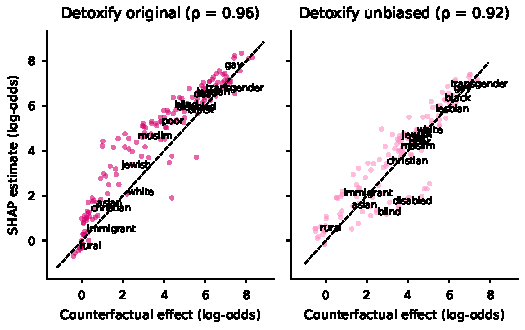
\includegraphics[width=\columnwidth]{fig_exp3_cf_vs_shap.pdf}%
}{%
  \fbox{\parbox{0.9\columnwidth}{\centering\vspace{1.5cm}Fig.~1 placeholder: copy fig\_exp3\_cf\_vs\_shap.pdf into paper/figures/\vspace{1.5cm}}}%
}
\caption{SHAP's estimate of each identity word's effect vs.\ its counterfactual effect (log-odds), one point per identity sentence ($n=150$). Dashed line: $y=x$. \todo{finalise caption}}
\label{fig:cf}
\end{figure}

% Exp 4 column changed from "MAE vs exact" to "rho vs exact": Exp 4 has no
% LIME MAE, but has rho for both explainers (exp4_summary.csv).
\begin{table}[t]
\caption{Faithfulness summary \todo{check values and finalise caption}}
\label{tab:faith}
\centering
\footnotesize
\setlength{\tabcolsep}{3pt}
\begin{tabular}{@{}lcccc@{}}
\toprule
 & $\rho$ vs.\ CF & $\rho$ vs.\ exact & Comp.\ $\uparrow$ / Suff.\ $\downarrow$ & Top word changes \\
 & (Exp 3, orig/unb) & (Exp 4, low/high) & (Exp 5, orig) & (Exp 6, 5000) \\
\midrule
SHAP   & 0.96 / 0.92 & 1.00 / 0.99 & 3.09 / $-2.43$ & n/a \\
LIME   & 0.97 / 0.97 & 1.00 / 0.98 & 3.05 / $-2.65$ & 4\% \\
Random & n/a & n/a & 0.35 / 1.30 & n/a \\
\bottomrule
\end{tabular}
\end{table}

\subsection{Deletion Test}
% Exp 5 (Bláithín). Sources: exp5_aopc.csv, exp5_aopc_by_group.csv.
% Negative sufficiency is only reported here; it is explained in Section V.
Deleting the top-ranked words lowered the toxic log-odds far more than deleting random words (Table~\ref{tab:faith}). Comprehensiveness was 3.09 for SHAP and 3.05 for LIME vs.\ 0.35 for random words with the original model, and 4.02, 4.06 and 0.95 with the unbiased model. The gap over random was largest on the Experiment~1 counter and report sentences (4.58 and 4.52 log-odds for SHAP, original model) and smallest on the control sentences, where comprehensiveness was close to zero for every explainer (SHAP $-0.02$, LIME 0.01). Sufficiency was negative for both explainers: $-2.43$ for SHAP and $-2.65$ for LIME with the original model, and $-0.97$ and $-0.85$ with the unbiased model, against $+1.30$ and $+2.63$ for random words. So keeping only the top-ranked words gave a higher toxicity score than the full sentence. The effect was strongest on report sentences ($-3.4$ for both explainers, original model).

\subsection{Where the Explainers Break}
\begin{itemize}
  \item Fig.~\ref{fig:stability} goes here. $n = 238$ sentences $\times$ 10 seeds. Sources: \texttt{exp6\_summary.csv}, \texttt{exp6\_stability\_by\_sentence.csv}, \texttt{exp6\_warning\_signs.csv}.
  \item Top word changed between seeds in 12\% of sentences at 500 samples, 4\% at 5000; mean rank stability 0.96 / 0.99.
  \item Instability vs.\ signal strength: $\rho = 0.04$ / 0.03, i.e.\ no relationship (Fig.~\ref{fig:stability} is a flat cloud, and that is the result).
  \item But fit drops on weak signals: $\rho(\text{signal}, R^2) = 0.73$; mean $R^2 \approx 0.45$ on the weakest quarter vs.\ 0.87 on the strongest; top-word agreement with SHAP 0.86 vs.\ 0.94.
  \item Warning signs for the worst 25\% of SHAP errors ($n=150$ identity sentences), AUC: SHAP--LIME disagreement 0.46, low $R^2$ 0.64, weak signal 0.80.
  \item Decide: keep Fig.~\ref{fig:stability} as is, or replot as $R^2$ vs.\ signal (EXP6 Cell 7). Caption must match either way.
\end{itemize}

\begin{figure}[t]
\centering
\IfFileExists{figures/fig_exp6_instability_vs_signal.pdf}{%
  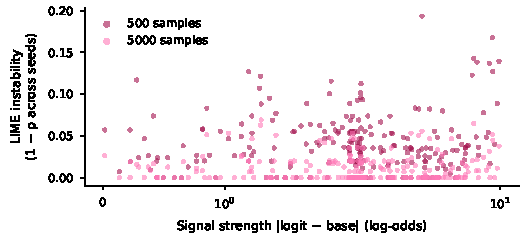
\includegraphics[width=\columnwidth]{fig_exp6_instability_vs_signal.pdf}%
}{%
  \fbox{\parbox{0.9\columnwidth}{\centering\vspace{1.5cm}Fig.~2 placeholder: copy fig\_exp6\_instability\_vs\_signal.pdf into paper/figures/\vspace{1.5cm}}}%
}
\caption{LIME instability across 10 seeds vs.\ signal strength, at 500 and 5000 samples ($n=238$ sentences). \todo{finalise caption}}
\label{fig:stability}
\end{figure}

\subsection{Sensitivity to the Removal Baseline}
\begin{itemize}
  \item 2--3 sentences with numbers. Sources: \texttt{exp3\_baselines.csv}, \texttt{exp3\_baseline\_rankings.csv}.
  \item Term ranking barely changes across dots / delete / mask: $\rho \geq 0.97$ for every pair, both models.
  \item Magnitudes do change: MAE 0.94 $\rightarrow$ 0.84 $\rightarrow$ 0.70 (original), 0.72 $\rightarrow$ 0.58 $\rightarrow$ 0.44 (unbiased); control-word $|\phi|$ (original) 0.64 $\rightarrow$ 0.43 $\rightarrow$ 0.39.
\end{itemize}

% ---------------------------------------------------------------------
% V. DISCUSSION AND CRITICAL ANALYSIS (about 0.4 page)
% Owner: Julia
%
% FIRST DRAFT (2026-10-21).
% ---------------------------------------------------------------------
\section{Discussion}\label{sec:discussion}

\todo{}

\subsection{Gets order of identity terms right, not exactly how big their effects are:}
\begin{itemize}
  \item Counterfactual effect (true answer): Swap identity word (e.g. gay) for a neutral control word (e.g. tall) and measure how much the Detoxify score changes, in log-odds. Only one word changes, so that change is caused by that word.
  \item SHAP's estimate: what SHAP says that word contributed
  \item Evidence: Experiment 3
  \item A high p (Spearman's rank correlation: measures how similar two rankings are, rank by true counterfactual effect, rank same terms by SHAP's number, p measures how closely they line up) can be inflated by the wide spread between strong identity terms and near-zero control terms.
  \item An auditor needs magnitudes not just rankings, SHAP is good for flagging which terms to look at, but weaker for ``this filter's bias is X big''
\end{itemize}

\subsection{SHAP overstates the identify/counterfactual effect}
\begin{itemize}
  \item Based off experiment 3 results an attribution-based audit would overstate bias here. Safer than understating, but still wrong
\end{itemize}

\subsection{``Debiased'' doesn't mean identity-insensitive}
\begin{itemize}
  \item Gap between what the ``unbiased'' label on Detoxify promises and what our experiment actually tests
  \item Detoxify unbiased was trained to be fair on average across many real comments (\textbf{Borkan 2019}), it wasn't trained to give the same score when you swap the group word in a single sentence (\textbf{Garg 2019}). That's why it can be called ``unbiased'' and still react strongly to ``gay'' in our tests (can be unbiased by one definition and biased by another).\newline
  For example: A teacher takes 10 marks off every essay by one group. Within that group, good essays still beat bad ones, so ordering is fine and Test 1 is passed. Swap the name on any single essay and the mark jumps 10 points so Test 2 is failed. Detoxify unbiased was trained to pass Test 1, not Test 2.
  \item Explains our weird looking result and shows that someone must choose what ``fair'' means.
\end{itemize}

\subsection{Rudin's Debate}
\begin{itemize}
  \item How much worse is our simple model in comparison to detoxify:\newline
  -AUC measures how well a filter separates toxic from non-toxic comments (1.0 = perfect, 0.5 no better than random). Experiment 4 results: there's a small gap between but not enough than an auditor couldn't reasonably argue for the simple model
  \item Simple model is biased too, since it's transparent we can read the score it gave each word, bias didn't come from the design but rather the training data. A simple model lets us see this directly. Rudin's approach makes bias easy to spot, but it doesn't fix it.
\end{itemize}

\subsection{Triage vs Certify}
\begin{itemize}
  \item In an audit a false negative is much worse than a false positive. SHAP/LIME are reliable on strong signals, weak on weak signals (experiment 6) and can be gamed adversarially (Slack 2020).
  \item Experiment 6: Which warning signs predict the worst 25\% of SHAP errors against the true answer? Weak signal strength etc
\end{itemize}

\subsection{Agreeing and Repeating is not equal to being right}
\begin{itemize}
  \item SHAP and LIME aren't independent witnesses. Both explain by removing words, so they share the same out-of-distribution bias and their errors are likely correlated. Agreement cant serve as validation (Krishna 2022).
  \item LIME on weak signals is consistent but consistently a poor fit. Fit and agreement fall on weak signals. On weak signals LIME gives the same answer every run, but that answer comes from a surrogate that explains under half the variance.
\end{itemize}

\subsection{Explanations can't decide what ``fair'' means}
\begin{itemize}
  \item Faithful to the model doesn't mean right about the world. The glass-box coefficients show that ``gay'' is associated with toxicity in Civil Comments labels. SHAP describes that faithfully. Whether removing such text is a harm is a normative question about whos language counts (Gururangan, 2022)
  \item Not causal in the world. The counterfactual swap is causal within the model. It says nothing about downstream harm, which communities vanish from the corpus or what the LLM then learns.
\end{itemize}

% ---------------------------------------------------------------------
% VI. CONCLUSION AND LIMITATIONS (about 0.25 page)
% Owner: Rory Linnane
% ---------------------------------------------------------------------
\section{Conclusion and Limitations}\label{sec:conclusion}

We tested whether SHAP and LIME can support a social-bias audit of a pretraining data filter.
Our experiments show that both explainers are faithful enough to be useful: they identify words that genuinely drive removal decisions, with deletion of SHAP's top-3 tokens causing a mean log-odds drop of 3.09 versus 0.35 for random tokens, and their attributions align with counterfactual identity-swap effects and with exact Shapley values on a transparent filter.
However, faithfulness is not uniform: stability degrades on weak-signal sentences, attributions shift with the choice of removal baseline, and the two explainers disagree more often than their overall agreement rate implies~\cite{krishna2022disagreement}.
We therefore recommend that auditors use attribution as a triage tool --- to flag suspicious filter behaviour for further review --- rather than as a certification of fairness.
In practice: (1)~report LIME's surrogate $R^2$ and re-run with multiple seeds to check stability; (2)~treat high SHAP--LIME disagreement as a signal for human review; (3)~confirm any attribution finding with a counterfactual swap before drawing conclusions.

\smallskip
\noindent\textbf{Limitations.}
Our scope is purposely narrow: we use short English template sentences with single word identity substitutions, which do not capture dialect-level bias (e.g.\ AAE~\cite{sap2019risk}) where no single word carries the signal.
We test one filter family (Detoxify \texttt{original} and \texttt{unbiased}), and the two models differ in architecture (BERT vs.\ RoBERTa) as well as debiasing objective, so architectural effects cannot be fully separated.
The transparent filter in Experiment~4 is our own construction, not a real pipeline filter.
Our ground-truth references --- counterfactual effects and exact Shapley values --- exist only because we controlled the inputs; a real auditor facing an opaque commercial filter would not have them.
We did not evaluate quality filters, blocklists, or non-English data.

\smallskip
\noindent\textbf{Future work.}
Extending attribution audits to real web text from C4 or Common Crawl, to the quality filter of~\cite{gururangan2022whose}, and to human rationale benchmarks such as HateXplain~\cite{ngueajio2025decoding} would address the most significant scope limitations.


% Spec: references go on their own page.
\clearpage

\bibliographystyle{IEEEtran}
\bibliography{refs}

\end{document}
